%!TEX root = /Users/bilalh/Uni/CS/SH/CS4102-CG/Practicals/CS4102-CG-P5/Practical5/report/Main.tex

\section{Introduction} % (fold)
\label{sec:introduction}
My solution implements all the required features of the practical and also implements all the extensions plus some extra features.

% section introduction (end)

\section{Usage} % (fold)
\label{sec:usage}
The program can be run by opening it in Xcode and running it. The program was tested using Xcode 4 on Mac OS X 10.6.8. There is also a video, \texttt{Practical5.mp4} of the program running.
% section usage (end)

\section{Implementation}

\begin{figure}[htbp]
	\centering
		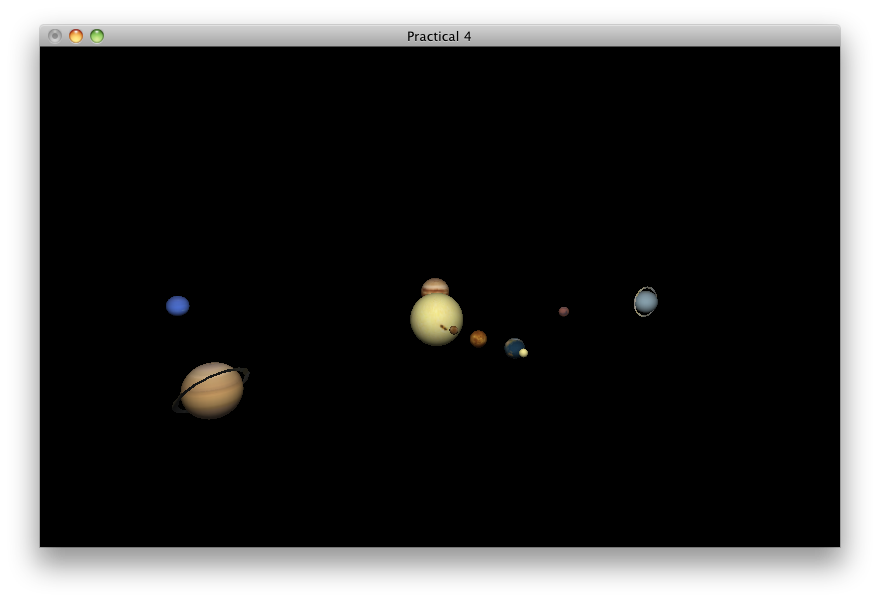
\includegraphics[width=6.7in]{figures/main.png}
	\caption{Shows all the planets, the earth has a moon orbiting it. Saturn and Uranus have rings around them.}
	\label{fig:main}
\end{figure}

\def\fp{0.3}
\begin{figure}[p]
	\subfigure[Top Down View with Orbits turned on.]{
		\label{fig:show1} 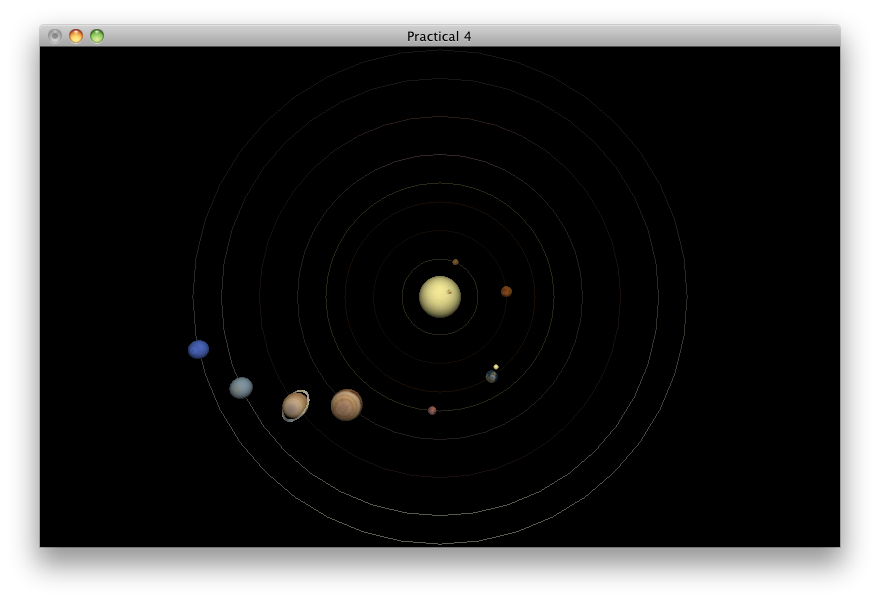
\includegraphics[scale=\fp]{figures/f1.png}} 
	\subfigure[Different lighting, shows the rings of the Saturn and Uranus.]{
		\label{fig:show2} 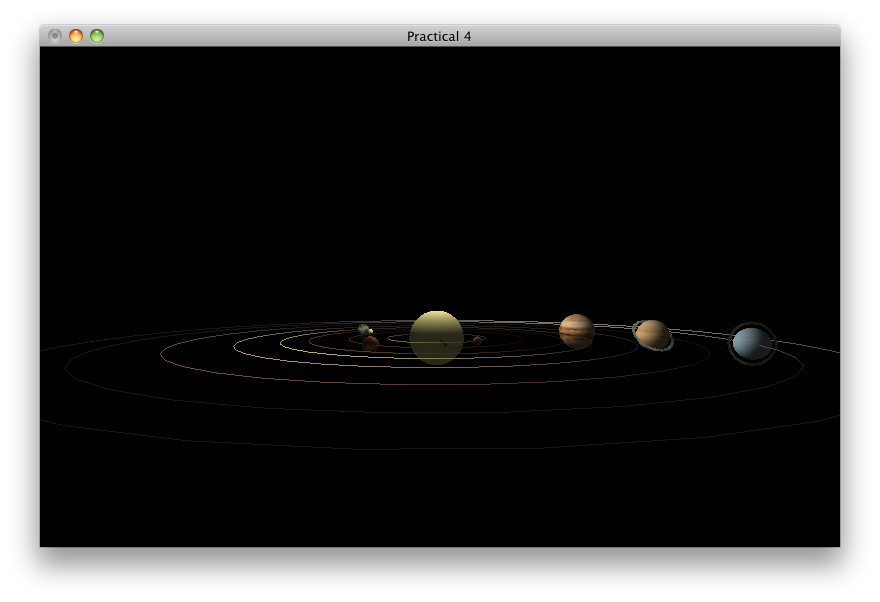
\includegraphics[scale=\fp]{figures/f2.png}} 
	\subfigure[Shows the camera attached to a planet.]{
		\label{fig:show3} 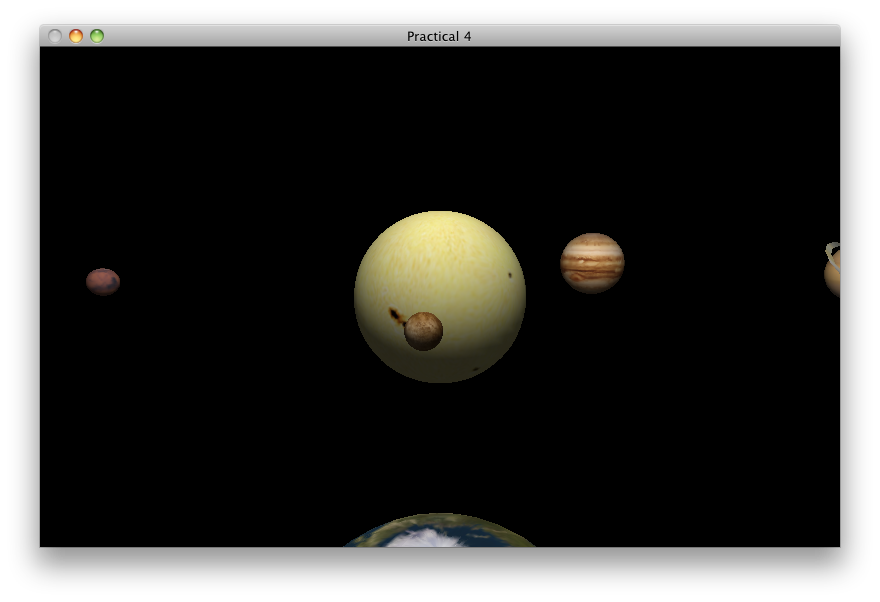
\includegraphics[scale=\fp]{figures/f3.png}} 
	\subfigure[No lighting.]{
		\label{fig:show4} 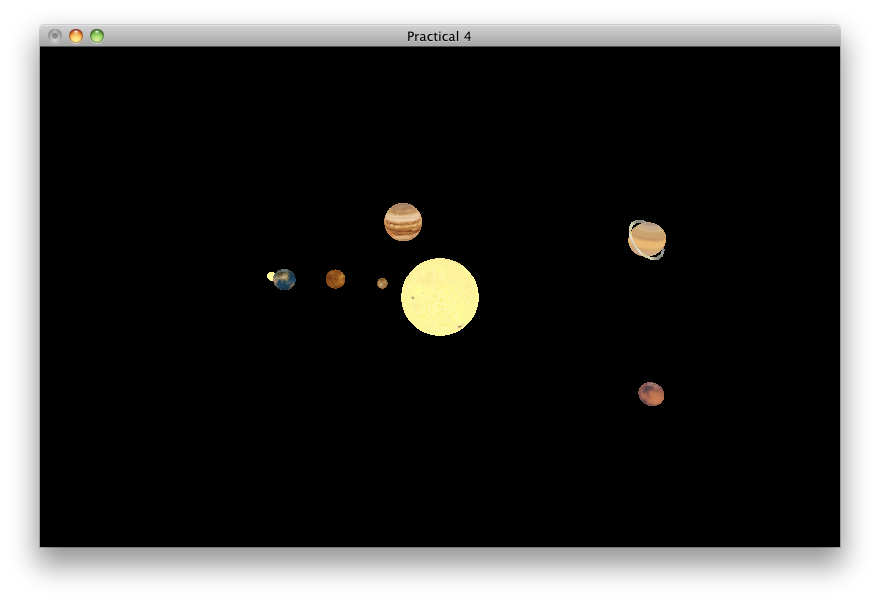
\includegraphics[scale=\fp]{figures/f4.png}} 
	\subfigure[Side view, Most of the planets are hidden by the sun.]{
		\label{fig:show5} 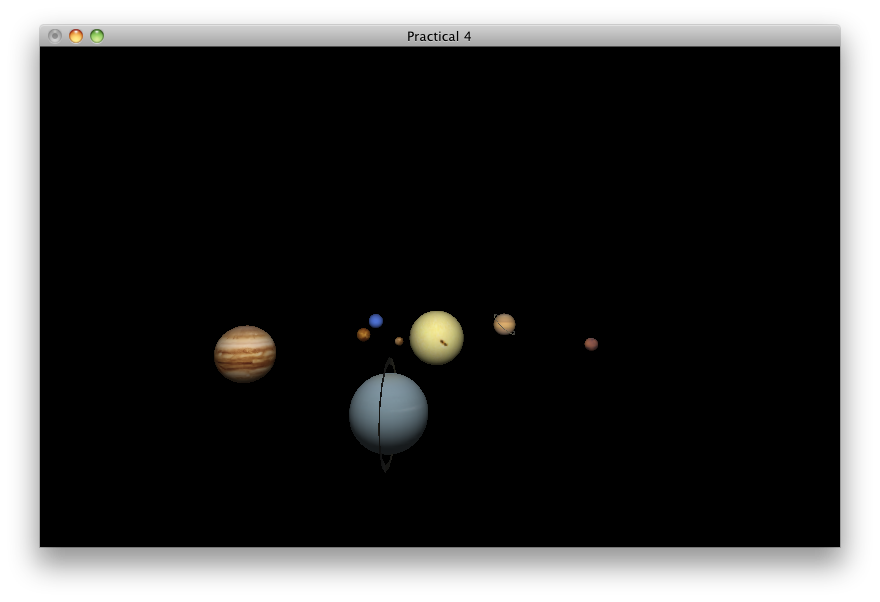
\includegraphics[scale=\fp]{figures/f5.png}} 
	\subfigure[The materials of some of the planets have also been changed. ]{
		\label{fig:show6} 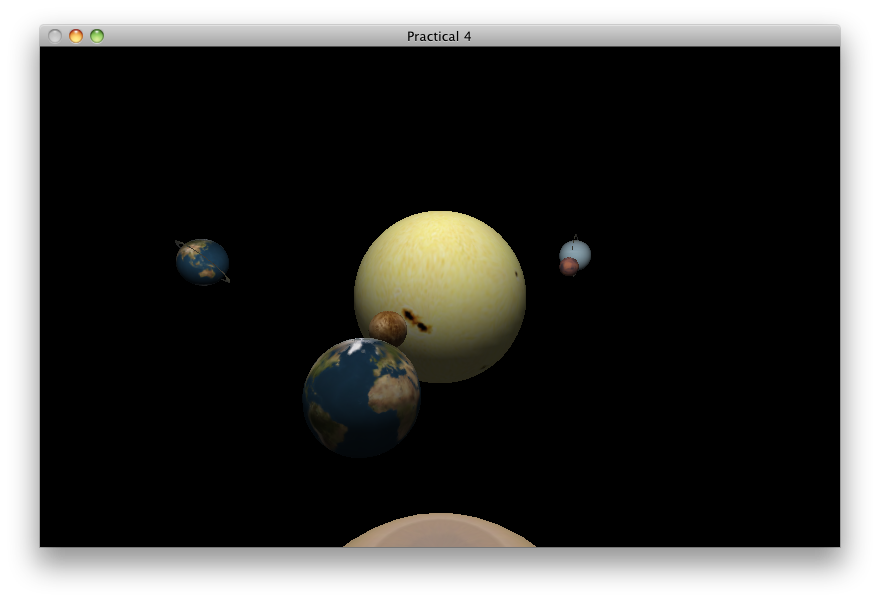
\includegraphics[scale=\fp]{figures/f6.png}}
\end{figure}

\clearpage
The solution has the key binding specified in Practical 4  plus extra keybindings. The solution also handles window resizing on which more/less of the model is shown. The speed that the planets move can be increased or decreased using the `\texttt{-}' or `\texttt{+}' keys. `\texttt{l}' goes through different lighting configurations (including no lighting). `\texttt{v}' goes through a series of predefined viewports. The spacebar toggles the movement of the planets and  \texttt{[} and \texttt{]} can be used to zoom out/zoom in.
 
The textures of the planets can be done either by right clicking or clicking on a planet then pressing `\texttt{m}' as shown in figure \ref{fig:show6}. The textures were taken from \cite{pp} and loaded from jpegs using \texttt{libjpeg}. \texttt{libjpeg} was complied from source for Mac OS X 10.6.8 (64bit) and is induced in the \texttt{libjpeg} directory so that the solution can run on other computers.  

The camera can be attached to planet as shown in figure \ref{fig:show3}, this is done by clicking on a planet then pressing `\texttt{a}', The camera can rotate when attached to a planet as shown below, by using the arrow keys. 

	\begin{figure}[htbp]
		\centering
			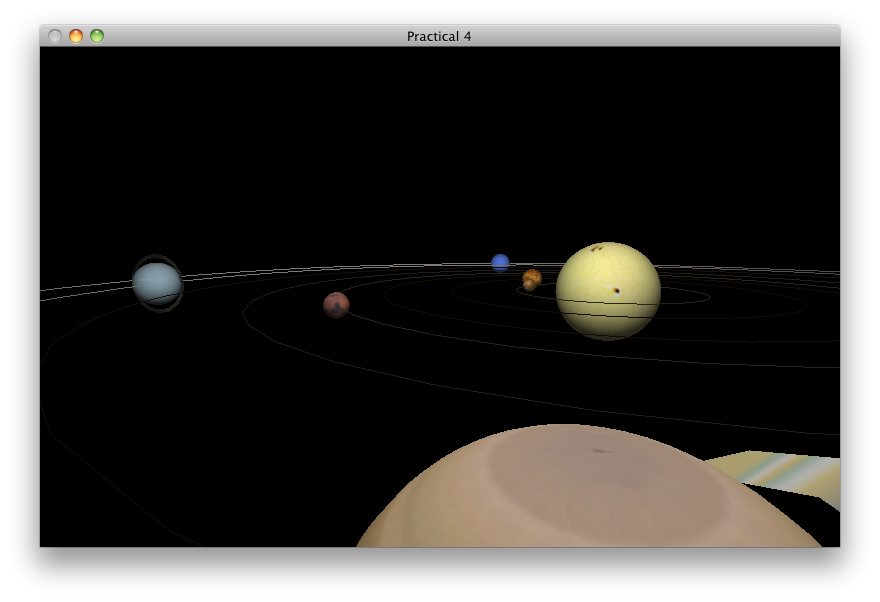
\includegraphics[scale=0.4]{figures/a.png}
		\caption{Shows the circling camera when using the arrow keys after attaching the camera to Saturn. }
		\label{fig:main}
	\end{figure}

All the planets (and the moon) rotate as they move around their orbit, Saturn and Uranus have rings around them. The solution uses a hierarchical model that allows modelling of an aberrantly Solar System.  

The model allows planets to have other celestial bodies orbiting them. Planets can have any number of \texttt{Drawable} objects attached to them, which allows rings around the planets.

\section{Video} % (fold)
\label{sec:video}
The video shows the features of the program, the viewpoints, rotating planets as they orbit, showing/hide orbits, the different lighting configurations, changing the textures of the planets and also shows attaching the camera to different planets. It also shows zooming in/zooming out. 


% section video (end)